\documentclass{amsart}
\usepackage[margin=3cm]{geometry}                % See geometry.pdf to learn the layout options. There are lots.
\geometry{letterpaper}                   % ... or a4paper or a5paper or ...
%\geometry{landscape}                % Activate for for rotated page geometry
\usepackage[parfill]{parskip}    % Activate to begin paragraphs with an empty line rather than an indent
\usepackage{float}
\usepackage{graphicx}
\usepackage{amssymb}
\usepackage{epstopdf}
\usepackage{siunitx}
\usepackage{subcaption}
\usepackage{listings}

\DeclareGraphicsRule{.tif}{png}{.png}{`convert #1 `dirname #1`/`basename #1 .tif`.png}
\graphicspath{{./img/}}

\title{Swinging Gate Pendulum Seismometer}
\author{Caspar \textsc{Lant}} % Author name

\date{\today} % Date for the report

\begin{document}

\bigskip

\maketitle % Insert the title, author and date
\begin{center}

Intermediate Experimental Physics II\\
\vspace{1.5cm}

\begin{tabular}{l r}

Section: & 002\\
\\
Date Performed: & February 16, 2016 \\ % Date the experiment was performed
Date Due: & February 23, 2016\\
\\
Partner: & Neil Saddeler\\ % Partner names
Professor: & Prof. Andrew Kent\\
Instructor: & David Mykytyn % Instructor/supervisor
\end{tabular}
\end{center}
\vspace{50mm}
\pagebreak

\paragraph{\textbf{The Objective} of this week's experiment was to put our vast theoretical knowledge of lenses to application. It is always a remarkable think to see what was once pure abstraction validated though rigorous scientific experimentation. }

\section{Theoretical Background/ Abstract}
\paragraph{Lenses have been of interest to us humans for a long time now. Convex lenses, concave lenses, even planar mirrors have all been the subjects of frenzied study through the ages. This should come as no surprise, given how fantastically useful they are to creatures who experience the world, mainly, through sight. We are mainly interested in what happens to the light from objects in front of the lens}
\begin{equation}
\frac{1}{s_i}+ \frac{1}{s_o} = \frac{1}{f}
\end{equation}
\begin{equation}
\frac{1}{f} = (n-1)\Big(\frac{1}{R_1} - \frac{1}{R_2}\Big)
\end{equation}

\section{Experimental Procedure}
\begin{enumerate}
\item Level the seismometer by adjusting the thumbscrew on its base. It turns out that the best way to do this is not with the provided bubble level, but by eye. You should dial adjust the screw to a height such that the device's pendulum finds its equillibrium position at the middle of the seismometer base.
\item Turn on data studio and set up a display of pendulum position versus time.
\item
\item
\item
\item
\item
\item
\item
\item
\item
\item
\item
\item
\end{enumerate}

\newpage
\lstinputlisting[language=Python]{./data/ReadDataFitPlot.py}
\newpage

\section{Graphs and Tables}

\begin{figure}
    \begin{minipage}{.45\textwidth}
        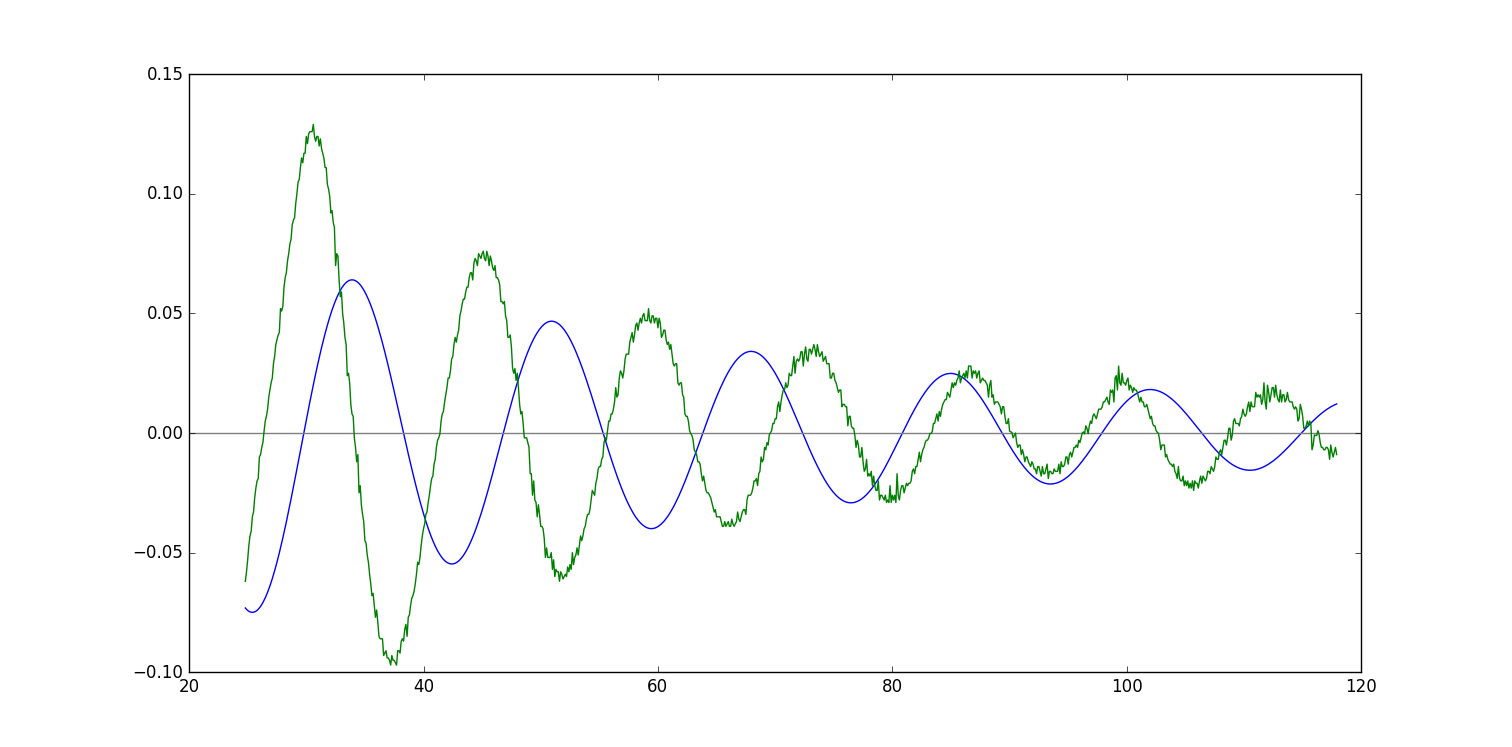
\includegraphics[width=\textwidth]{blow5.png}
        \caption{blow 5}
    \end{minipage}
    %
    \begin{minipage}{.45\textwidth}
        hello
    \end{minipage}
\end{figure}

\section{Questions}

\begin{enumerate}
\item {\textit{Question?}
\begin{quote}
Answer
\end{quote}}

\item{\textit{Repeat your measurements both with and without the vibration isolation mounts for the wooden table. Do you see a difference? Why or why not?}
\begin{quote}
Answer
\end{quote}}

\end{enumerate}

\section{Error Analysis}




\end{document}
